\section{Mendelian Imputation}

\subsection{Family Genome-Wide Association Studies (FGWAS)}

% Introduction to FGWAS
\begin{frame}{Why use them?}
    \begin{columns}
        % Column 1: Image
        \begin{column}{0.45\textwidth}
            \begin{figure}
                \centering
                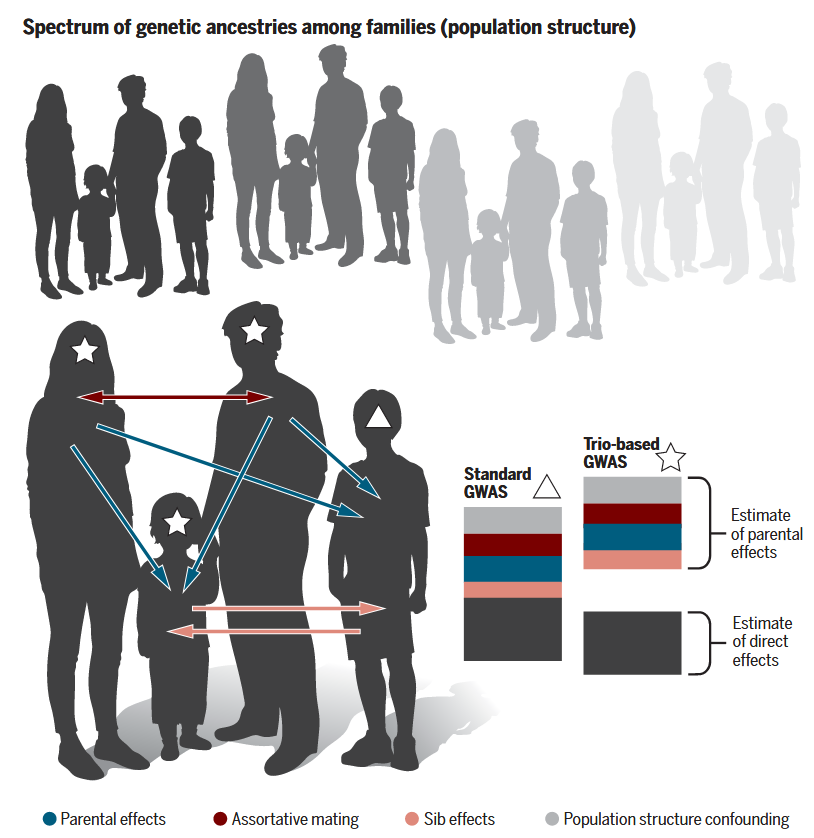
\includegraphics[height=2.15in]{young2022/fgwas-interactions.png}
                \caption{Signals captured by FGWAS in families \parencite{young2019}.}
                \label{fig:fgwas-genetic-signals}
            \end{figure}
        \end{column}

        % Column 2: Text
        \begin{column}{0.45\textwidth}
            % Block 1: 
            \begin{exampleblock}{Unbiased GWAS}<2->
                \begin{itemize}
                    \item<2-> Can discriminate \textbf{DGEs}\footnote{Direct Genetic Effects} and \textbf{Population Effects} using \textbf{parental genotypes} as controls.
                    \item<3-> Source of genetic variation is \textbf{\textit{within-family}}.
                \end{itemize}
            \end{exampleblock}

            % Block 2
            \begin{alertblock}{We lose power}<4->
                \begin{itemize}
                    \item<4-> We need \textbf{more individuals $n$} to be genotyped.
                    \item<5-> Complete parent-offspring trios are \textit{rare} in cohorts.
                \end{itemize} 
            \end{alertblock}
        \end{column}
    \end{columns}
\end{frame}


